\documentclass[../note.tex]{subfiles}

\begin{document}

\section{구간}
\subsection{정의}
\begin{definition}[구간]

  구간\textsuperscript{interval}. 단어에서 유추되는 바와 같이 특점 원소 사이를 말한다. $-1$과 $1$ 사이에는 무수히 많은 실수가 존재하는데, $-1$과 $1$ 사이의 `구간'은 이를 모두 망라하기에 구간은 하나의 집합이다. 구간의 집합은 대개 연속되고 값의 크기가 비교되는 특징을 지닌다. i.e., 순서를 가진다.
\end{definition}
\begin{note}[구간의 원소가 순서를 가지지 않는다면?]
  예컨대 순서가 정의되지 아니한 복소수에서는 구간을 어떻게 표현할 수 있을까? $(3i, 5i)$와 같이 표현할 수 있을까? 이는 $3i$ 보다 크고 $5i$ 보다 작은 원소들의 집합을 의미해야 하는데, 복소수값은 대수 관계가 정의되지 아니하니 모순된다. 그러면 복소수 평면의 구간은 어떻게 표현할까? stackExchange에 등록된 질문\footnote{https://math.stackexchange.com/questions/899077/is-there-an-interval-notation-for-complex-numbers}에 따르면 복소수에서 구간은 다음과 같이 표현 가능하다:
  \begin{equation}
    [a, b] + [c, d]i
  \end{equation}
\end{note}

\subsection{구간의 종류}
다음은 구간의 종류이다. 구간은 끝점의 포함 여부에 따라 분류된다.
\begin{note}[구간의 종류]
  구간의 종류를 아래와 같이 표로 정리하였다:
  \begin{table}[H]
    \centering
    \begin{tabular}{ c c c c }
      표현 & 조건 제시법 & 이름 & diagram \\
      \hline
      $(a, b)$ & $\{x : a < x < b\}$ & 열린 구간\textsuperscript{open interval, 개구간} & \begin{tikzpicture}[scale=0.2]
        \draw (-10,1) -- (5,1);
        \draw[fill=white] (-10,1) circle (0.25);
        \draw[fill=white] (5,1) circle (0.25);
      \end{tikzpicture} \\
      $[a, b]$ & $\{x : a \leq x \leq b\}$ & 닫힌 구간\textsuperscript{closed interval, 폐구간} & \begin{tikzpicture}[scale=0.2]
        \draw (-10,1) -- (5,1);
        \fill (-10,1) circle (0.25);
        \fill (5,1) circle (0.25);
      \end{tikzpicture} \\
      $(a, b]$ & $\{x : a < x \leq b\}$ & 반열린 구간\textsuperscript{half-open interval, 반개구간} & \begin{tikzpicture}[scale=0.2]
        \draw (-10,1) -- (5,1);
        \draw[fill=white] (-10,1) circle (0.25);
        \fill (5,1) circle (0.25);
      \end{tikzpicture} \\
      $[a, b)$ & $\{x : a \leq x < b\}$ & 반열린 구간\textsuperscript{half-open interval, 반개구간} & \begin{tikzpicture}[scale=0.2]
        \draw (-10,1) -- (5,1);
        \fill (-10,1) circle (0.25);
        \draw[fill=white] (5,1) circle (0.25);
      \end{tikzpicture} \\
      $(a, \infty)$ & $\{x : x > a\}$ & 열린 구간\textsuperscript{open interval} & 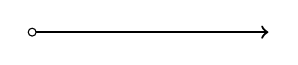
\begin{tikzpicture}[scale=0.2]
        \draw[->,thick] (-10,1) -- (5,1);
        \draw[fill=white] (-10,1) circle (0.25);
      \end{tikzpicture} \\
      $(\infty, b)$ & $\{x : x < b\}$ & 열린 구간\textsuperscript{open interval} & 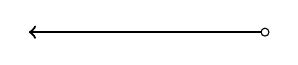
\begin{tikzpicture}[scale=0.2]
        \draw[<-,thick] (-10,1) -- (5,1);
        \draw[fill=white] (5,1) circle (0.25);
      \end{tikzpicture} \\
      $[a, \infty)$ & $\{x : x \leq a\}$ & 닫힌 구간\textsuperscript{closed interval} & 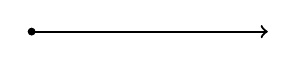
\begin{tikzpicture}[scale=0.2]
        \draw[->,thick] (-10,1) -- (5,1);
        \fill (-10,1) circle (0.25);
      \end{tikzpicture} \\
      $(-\infty, b]$ & $\{x : x \geq b\}$ & 닫힌 구간\textsuperscript{closed interval} & 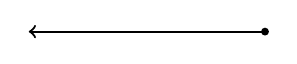
\begin{tikzpicture}[scale=0.2]
        \draw[<-,thick] (-10,1) -- (5,1);
        \fill (5,1) circle (0.25);
      \end{tikzpicture} \\
      $(-\infty, \infty)$ & $\RR$ & 실수 집합 & 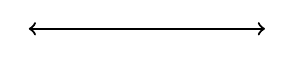
\begin{tikzpicture}[scale=0.2]
        \draw[<->,thick] (-10,1) -- (5,1);
      \end{tikzpicture} \\
   \end{tabular}
    \caption{구간의 종류}
  \end{table}
\end{note}

\epigraph{일반적으로 수학에서 구간이라고 말하면 열린 구간을 나타냅니다.}{--- 교수님}

\subsubsection{표현}
구간이 끝점을 포함하지 아니할 경우 `열린 구간'이라고 표현하며 기호 `$($'와 `$)$'로 표현한다. 반면 끝점을 포함하고 있을 경우 `닫힌 구간'이라고 표현하며 기호 `$[$'와 `$]$'로 표현한다.

\subsubsection{다이어그램}
구간이 끝점을 포함하지 아니하는 경우 다이어그램으로 표시할 때 포함하는 끝점을 안이 비어있는 점으로 표시하고, 끝점을 포함할 경우 안을 칠한 점으로 표시한다.

\begin{note}[구간에서의 무한대]
  왜 $(a, \infty)$ 등 한 끝점을 기준으로 하나의 방향으로 끝없이 연속되는 구간에서 $\infty$에 대하여 닫힌 구간으로 표현하지 않을까? $\infty$는 분명 하나의 숫자는 아니며 --- 그 어떤 실수 하나를 선택하여도 이는 $\infty$보다 작은 수이다 --- 순서 또한 정의되지 아니한다. 교수님은 수업 중 $\infty$는 하나의 `상태'라고 표현하였다. 닫힌 구간으로 표현하기 위해서는 구간의 끝 점이 구간에 포함되어야 하는데, 하나의 상태가 구간에 포함된다? 모순되고 어색하다.
\end{note}

\subsection{근방}
--- Mar 6에 추가함.
\begin{definition}[근방]
  점 $a$를 포함하는 집합 $N \subset \RR$을 점 $a$의 근방\textsuperscript{neighbourhood}라고 부른다. i.e.
  \begin{equation}
    a \in N \subset \RR
  \end{equation}

  단, neighbourhood는 일반적으로 open interval을 의미한다. open interval I에 대하여 다음과 같은 식을 찾을 수 있었다:
  \begin{equation}
    x \in I,\; I \subset N \Longleftrightarrow N \text{ is a neighbourhood of } x
  \end{equation}
\end{definition}
경우에 따라 적당한 근방을 찾아야 한다.

\section{특수한 집합의 표현}
고등학교 1학년 수업시간, 수학 선생님께서 해당 표현들을 알려주셨다. 개인적으로 큰 감명을 받았는데, 알다가도 모르겠는 `실수' 때문이었다: 1) `복소수가 아닌 수'라고 이해하기에는 정의가 아니라는 점. 2) 나머지, 예컨대 자연수와 유리수 등은 모두 실수에 조건을 주어 생성할 수 있다는 점. 그런데 실수 집합을 하나의 표현 $\RR$으로 나타내니 세상 고민 사라졌다.

\begin{note}[특수한 집합의 표현]
  집합은 다음과 같이 표현된다:
  \begin{table}[H]
    \centering
    \begin{tabular}{ c c }
      표현 & 의미 \\
      \hline
      $\NN$ & 자연수 집합 \\
      $\ZZ$ & 정수 집합 \\
      $\QQ$ & 유리수 집합 \\
      $\RR$ & 실수 집합 \\
      $\CC$ & 복소수 집합 \\
    \end{tabular}
    \caption{특수한 집합의 표현}
  \end{table}
\end{note}

\begin{itemize}
  \item
    $\NN$ : Natural number
  \item
    $\ZZ$ : Integer - I는 수학에서 많이 사용되는 문자이기에 --- 구간 또한 문자 $I$로 표현하는 경우가 허다하다 --- number를 뜻하는 독일어 `Zahlen'의 앞 글자를 따 $\ZZ$로 표현한다고 한다.
  \item
    $\QQ$ : Quotient
  \item
    $\RR$ : Real number
  \item
    $\CC$ : Complex number
\end{itemize}

해당 집합들은 실수 집합을 통해 정의 가능하다.

\begin{definition}
  실수 집합을 활용한 다른 집합의 정의:
  \begin{itemize}
    \item
      $\NN$\index{자연수 집합} : $\{x : x > 0,\; x \in \ZZ\}$
    \item
      $\ZZ$\index{정수 집합} : $\{x : x \mod 1 = 0,\; x \in \RR\}$
    \item
      $\QQ$\index{유리수 집합} : $\{x : x = \frac{p}{q},\; p, q \in \ZZ\}$
    \item
      $\CC$\index{복소수 집합} : $\{a+bi : a, b \in \RR\}$
  \end{itemize}
\end{definition}

정의에 따라 다음과 같은 포함 관계가 성립한다: $\NN \subset \ZZ \subset \QQ \subset \RR \subset \CC$

\section{양화사}
함수를 만족하기 위해서는 하나의 $x$값에 대하여 하나의 함숫값을 가져야 한다. 여기서, $x = 314$, $x = 421$ 등 특별한 $x$ 값에 대하여만 해당 조건이 만족하면 아니되고, 모든 $x$ 값에 대하여 만족하여야 한다. 이를 함수 $f(x):\RR->RR$에 대하여 다음과 같이 표현할 수 있다:
\begin{equation}
  \forall x_1, x_2 \in \RR : \left( f(x_1) = f(x_2) \right) \Longrightarrow \left( x_1 = x_2 \right)
\end{equation}
여기서 $\forall$는 전체 양화사라고 불리운다.

\begin{definition}[양화사]
  양화사\textsuperscript{quantifier}는 명제의 진위를 판단하는 데 사용되는 수식어이다. 양화사는 모든\textsuperscript{for all}과 어떤\textsuperscript{there exists}이 있다.
  \begin{table}[H]
    \centering
    \begin{tabular}{ c c }
      양화사 & 의미 \\
      \hline
      $\forall$\index{전체 양화사} & 모든 \\
      $\exists$\index{존재 양화사} & 어떤 \\
    \end{tabular}
    \caption{전체 양화사와 존재 양화사}
  \end{table}
\end{definition}

$\forall$은 All의 앞자인 A를 뒤집어 쓴 것이며, $\exists$는 존재의 앞자인 E를 뒤집어 쓴 것이다. 뒤집은 이유가 무엇인지 궁금하지만 기호를 처음 만든 사람이 문자와 구분되지만 의미를 쉽게 파악하기 위해 뒤집었다고 생각하고 넘어가겠다. (검색해도 이유를 잘 모르겠음)

이를 포함해 수학 문헌에서 다음과 같은 표현이 많이 사용된다.

\subsection{모든}
\begin{itemize}
  \item
    for all, for every
  \item
    for any, for arbitrary
  \item
    for each
\end{itemize}
\subsection{존재}
\begin{itemize}
  \item
    there exists, at least one
  \item
    there is
\end{itemize}

\end{document}
